\section{Hardware design of REACH}
In order to achieve our aforementioned vision we have augmented the sides of the mobile device with a total of 16 Force Sensitive Resistors (FSRs). These sensors change their resistance in response to the amount of force applied on them - the higher the force the lower the resistance. As shown in Figure \ref{fig:hardware_setup}, the sensors are split into two groups of 8, one grouping on each side of the device. The placement of these sensors has been optimized to ensure that a right-handed user has most contact with them while using the device. All the sensors are mounted onto a specially 3D printed case that house the acquisition electronics. A cable connects this setup to an Arduino Mega that handles the job of transferring the data to a Java application application running on a laptop. The hardware reads all sensor values at a rate of 1000 Hz. These values are then logged by the application for further processing.

\begin{figure}[h]
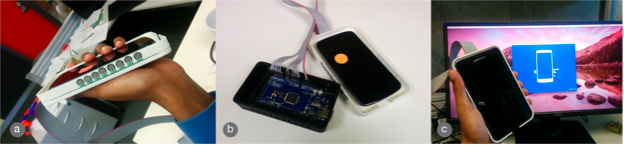
\includegraphics[width=.45\textwidth]{hardware_setup.png}
\caption{a) The sensors on the 3D printed case b) Connection to the Arduino c) A visualization of the force values}
\label{fig:hardware_setup}
\end{figure}
